\documentclass[11pt]{article}
\usepackage[a4paper,margin=1in]{geometry}
\usepackage{amsmath,amssymb,amsfonts}
\usepackage{booktabs}
\usepackage{graphicx}
\usepackage{caption}
\usepackage{enumitem}
\usepackage[table]{xcolor}
\usepackage{array}
\usepackage[hidelinks]{hyperref}
\usepackage{xurl}
\usepackage{microtype}

\title{2D Two-Target Double-Peak Conditions\\\large From Markov-Chain Derivation to Reflecting-Boundary Heatmap Validation}
\author{}
\date{}

\setlist{nosep}
\setlength{\textfloatsep}{8pt plus 2pt minus 2pt}
\setlength{\floatsep}{6pt plus 2pt minus 2pt}
\setlength{\intextsep}{6pt plus 2pt minus 2pt}
\setlength{\abovecaptionskip}{4pt}
\setlength{\belowcaptionskip}{0pt}
\setlength{\tabcolsep}{5pt}
\renewcommand{\arraystretch}{1.10}

\definecolor{fastcorr}{HTML}{CDE8F3}
\definecolor{slowcorr}{HTML}{E8E2AD}
\definecolor{overlapcorr}{HTML}{CDBFE2}
\definecolor{arrowred}{HTML}{FF5B4F}
\definecolor{lineblue}{HTML}{1F77B4}
\definecolor{lineorange}{HTML}{FF7F0E}
\definecolor{heatlow}{HTML}{2A0A8B}
\definecolor{heatmid}{HTML}{B5367A}
\definecolor{heathigh}{HTML}{FCD225}
\definecolor{phase0}{HTML}{E8E8E8}
\definecolor{phase1}{HTML}{9ECAE1}
\definecolor{phase2}{HTML}{FB9A99}

\newcommand{\legendbox}[1]{\fcolorbox{black}{#1}{\makebox[1.2em]{\rule{0pt}{0.9em}}}}
\newcommand{\legendline}[1]{\textcolor{#1}{\rule{2.0em}{0.8pt}}}

\begin{document}
\maketitle

\section*{Executive Summary}
This report addresses one question:
\textbf{under two absorbing targets in 2D, when does the total first-passage distribution show a visible double peak?}

Under reflecting boundaries and local-bias corridor design, the representative cases C1--C4 all show two modes in the total first-passage curve. The mechanism is:
\begin{enumerate}
  \item exact splitting decomposition of total first-passage, and
  \item sufficient mode separation with non-extreme splitting weights.
\end{enumerate}

\section{Mathematical Mechanism (From First Principles)}
\subsection{Single-step random walk definition}
On $\Omega=\{0,\ldots,N-1\}^2$ with $N=31$, the unbiased interior transition rule is
\begin{align}
P((x,y)\to(x\pm1,y))&=\frac{q}{4},\\
P((x,y)\to(x,y\pm1))&=\frac{q}{4},\\
P((x,y)\to(x,y))&=1-q.
\end{align}
We use $q=0.2$, hence each move direction is $0.05$ and stay probability is $0.8$.

Reflecting boundary means out-of-domain move mass is added back to stay probability.

\paragraph{Local-bias rule}
At a biased site, a fraction $\delta=0.2$ of the current stay probability is shifted to one arrow direction:
\begin{equation}
\Delta=\delta p_{\mathrm{stay}},\quad
p_{\mathrm{stay}}\leftarrow p_{\mathrm{stay}}-\Delta,\quad
p_{\mathrm{arrow}}\leftarrow p_{\mathrm{arrow}}+\Delta.
\end{equation}
For this setup, arrow-direction probability increases from $0.05$ to $0.21$, with effective drift
\begin{equation}
v_{\mathrm{eff}}\approx p_{\mathrm{forward}}-p_{\mathrm{backward}}=0.21-0.05=0.16 \text{ cells/step}.
\end{equation}

\subsection{Two-target absorbing Markov-chain block form}
Let $m_1,m_2$ be absorbing targets and $\mathcal T$ be transient states. With row-vector convention:
\begin{equation}
P=
\begin{bmatrix}
Q & R\\
0 & I_2
\end{bmatrix},\quad
R=[r_1\ r_2].
\end{equation}
Initial distribution is $\alpha$ (one-hot at $n_0$), and transient mass evolves as
\begin{equation}
u_0=\alpha,\qquad u_t=\alpha Q^t.
\end{equation}

\subsection{Exact splitting decomposition}
The splitting first-passage distributions are
\begin{equation}
f_1(t)=F_{n_0\to(m_1|m_2)}(t)=\alpha Q^{t-1}r_1,\quad
f_2(t)=F_{n_0\to(m_2|m_1)}(t)=\alpha Q^{t-1}r_2.
\end{equation}
Therefore total first-passage is exactly
\begin{equation}
F_{n_0\to(m_1;m_2)}(t)=f_1(t)+f_2(t)=\alpha Q^{t-1}(r_1+r_2).
\label{eq:split-sum-en}
\end{equation}

Survival and hazard:
\begin{equation}
S(t)=\alpha Q^t\mathbf 1,\qquad
h(t)=\frac{F_{n_0\to(m_1;m_2)}(t)}{S(t-1)}=\frac{f_1(t)}{S(t-1)}+\frac{f_2(t)}{S(t-1)}.
\end{equation}
Valleys occur when both channel contributions are simultaneously low.

\subsection{Generating-function form and practical criteria}
With $\tilde f(z)=\sum_{t\ge1}f(t)z^t$:
\begin{equation}
\tilde f_i(z)=z\,\alpha(I-zQ)^{-1}r_i,\qquad
\tilde F_{\mathrm{any}}(z)=\tilde f_1(z)+\tilde f_2(z).
\end{equation}
At $z=1$, splitting masses are
\begin{equation}
p_i=\sum_{t\ge1}f_i(t)=\alpha(I-Q)^{-1}r_i,\qquad p_1+p_2=1.
\end{equation}

In practice, visible double-peak behavior in $F_{\mathrm{any}}(t)$ needs:
\begin{itemize}
  \item sufficient mode separation, and
  \item non-negligible splitting weights for both channels.
\end{itemize}

\section{Model Setup and Real Heatmaps (Not Illustrative Templates)}
Fixed (1-based) coordinates:
$n_0=(15,15)$, $m_1=(22,15)$, $m_2=(7,7)$.
Fast centerline: $(15,15)\to(22,15)$.
Slow centerline:
$(15,15)\to(15,27)\to(3,27)\to(3,7)\to(7,7)$.

The yellow/purple corridor cells are biased cells.
In the compact overview figures, red arrows are centerline-sampled for readability.
The appendix provides full-arrow maps with one arrow for every biased cell.

\begin{figure}[!htbp]
  \centering
  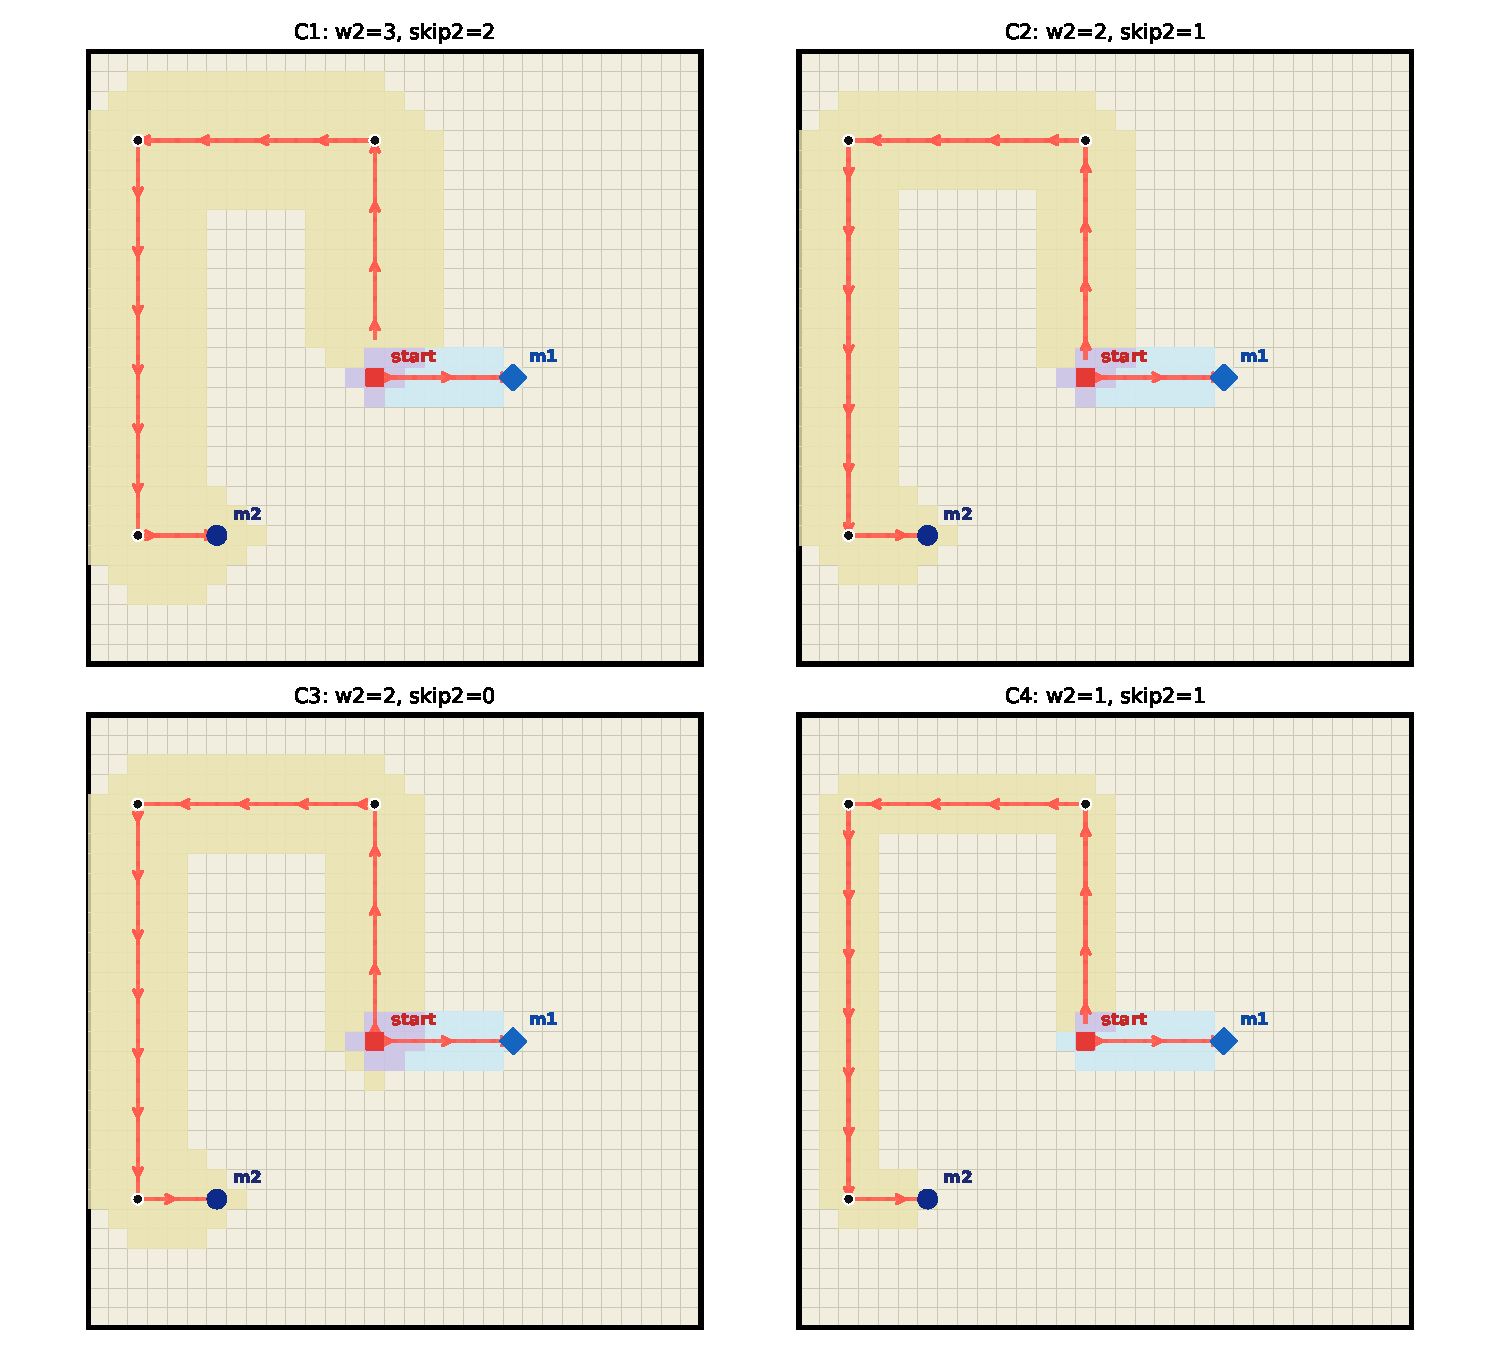
\includegraphics[width=0.90\linewidth]{figures/geometry_grid.pdf}
  \caption{Geometry overview for C1--C4: reflecting lattice background, fast/slow corridor cells, and transport-direction arrows.}
  \label{fig:geometry-grid-en}
\end{figure}

\begin{figure}[!htbp]
  \centering
  
\includegraphics[width=0.92\linewidth]{figures/symbol_legend_panel.pdf}
  \caption{Unified symbol legend panel generated by the same plotting pipeline.}
  \label{fig:symbol-legend-en}
\end{figure}

\begin{figure}[!htbp]
  \centering
  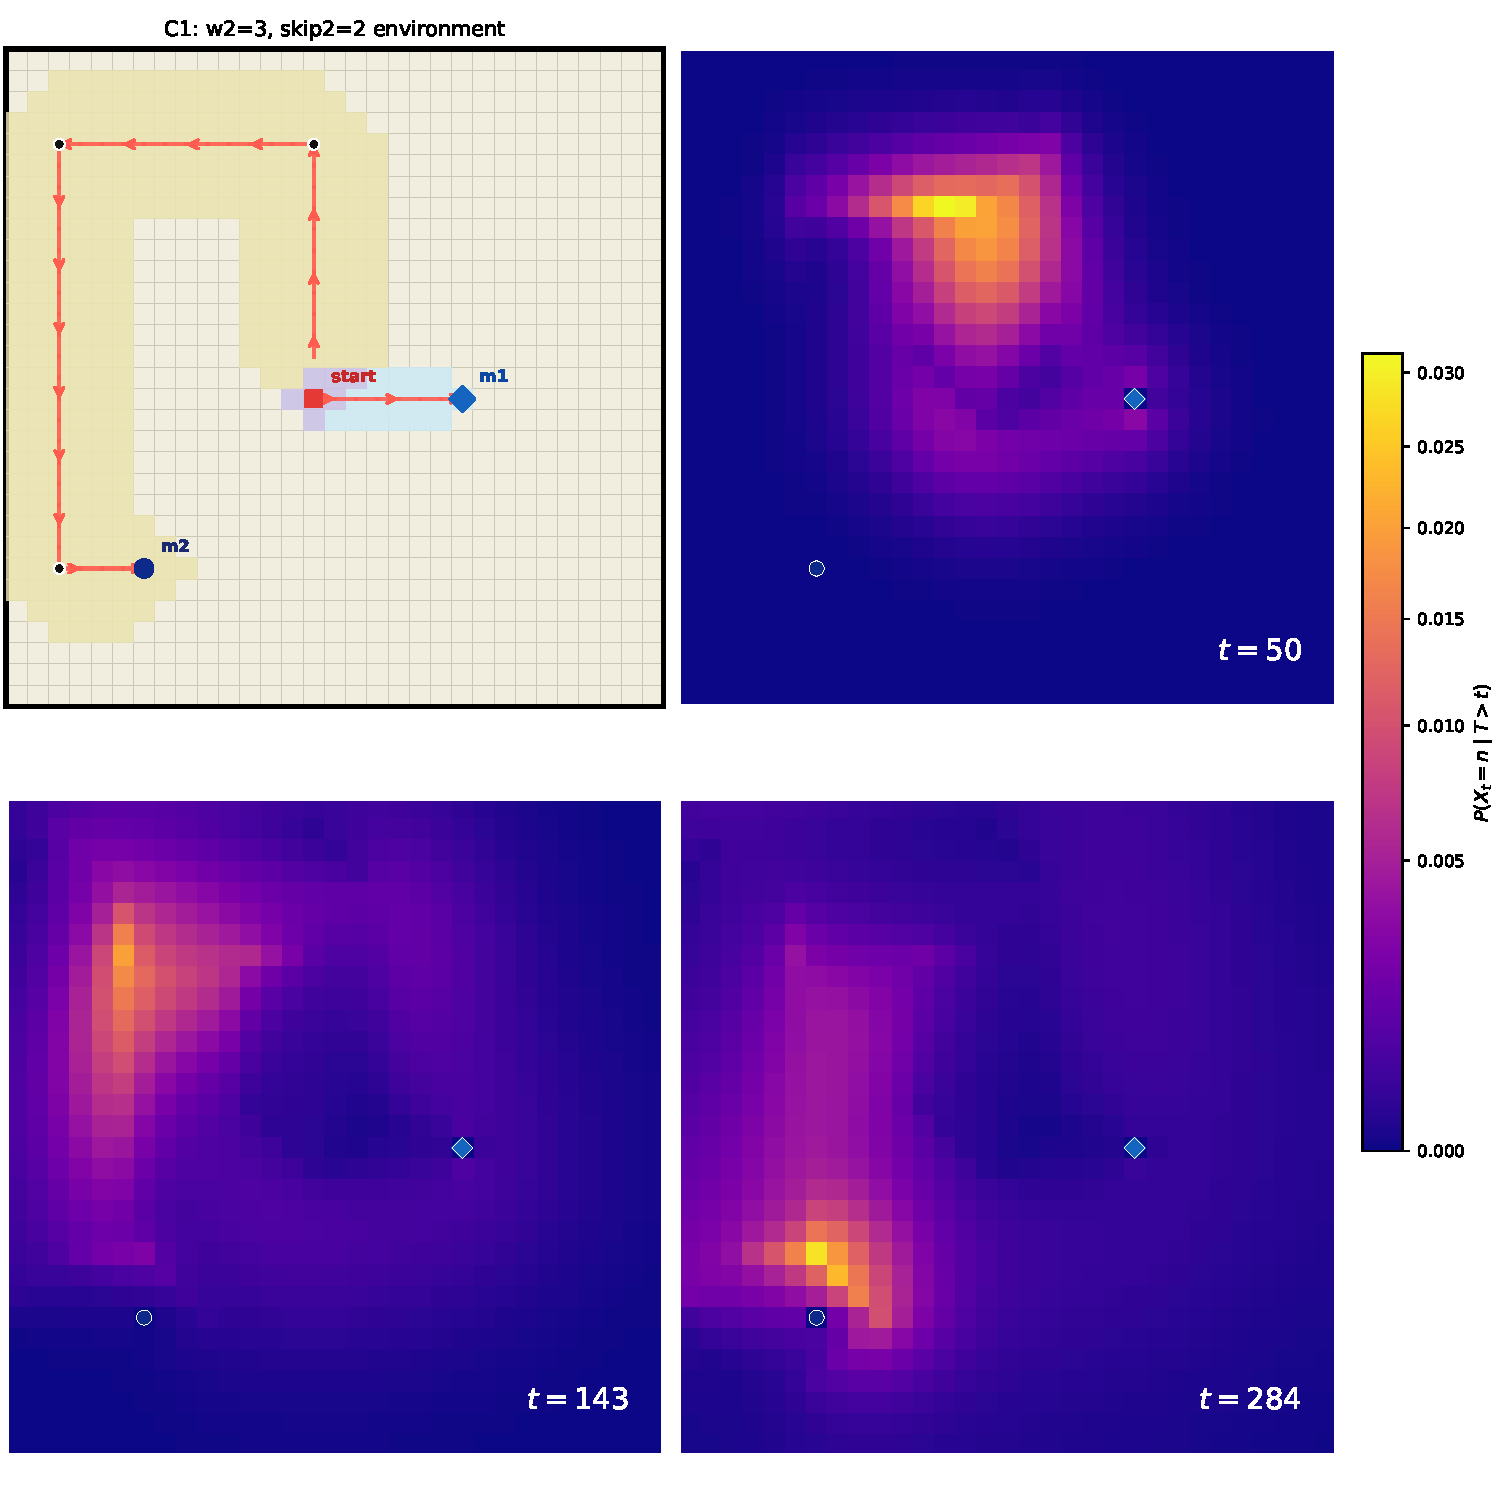
\includegraphics[width=0.82\linewidth]{figures/case_C1_env_heatmap.pdf}
  \caption{C1 environment + three computed conditional occupancy heatmaps ($t=50,143,284$).}
  \label{fig:c1-heat-en}
\end{figure}

\begin{figure}[!htbp]
  \centering
  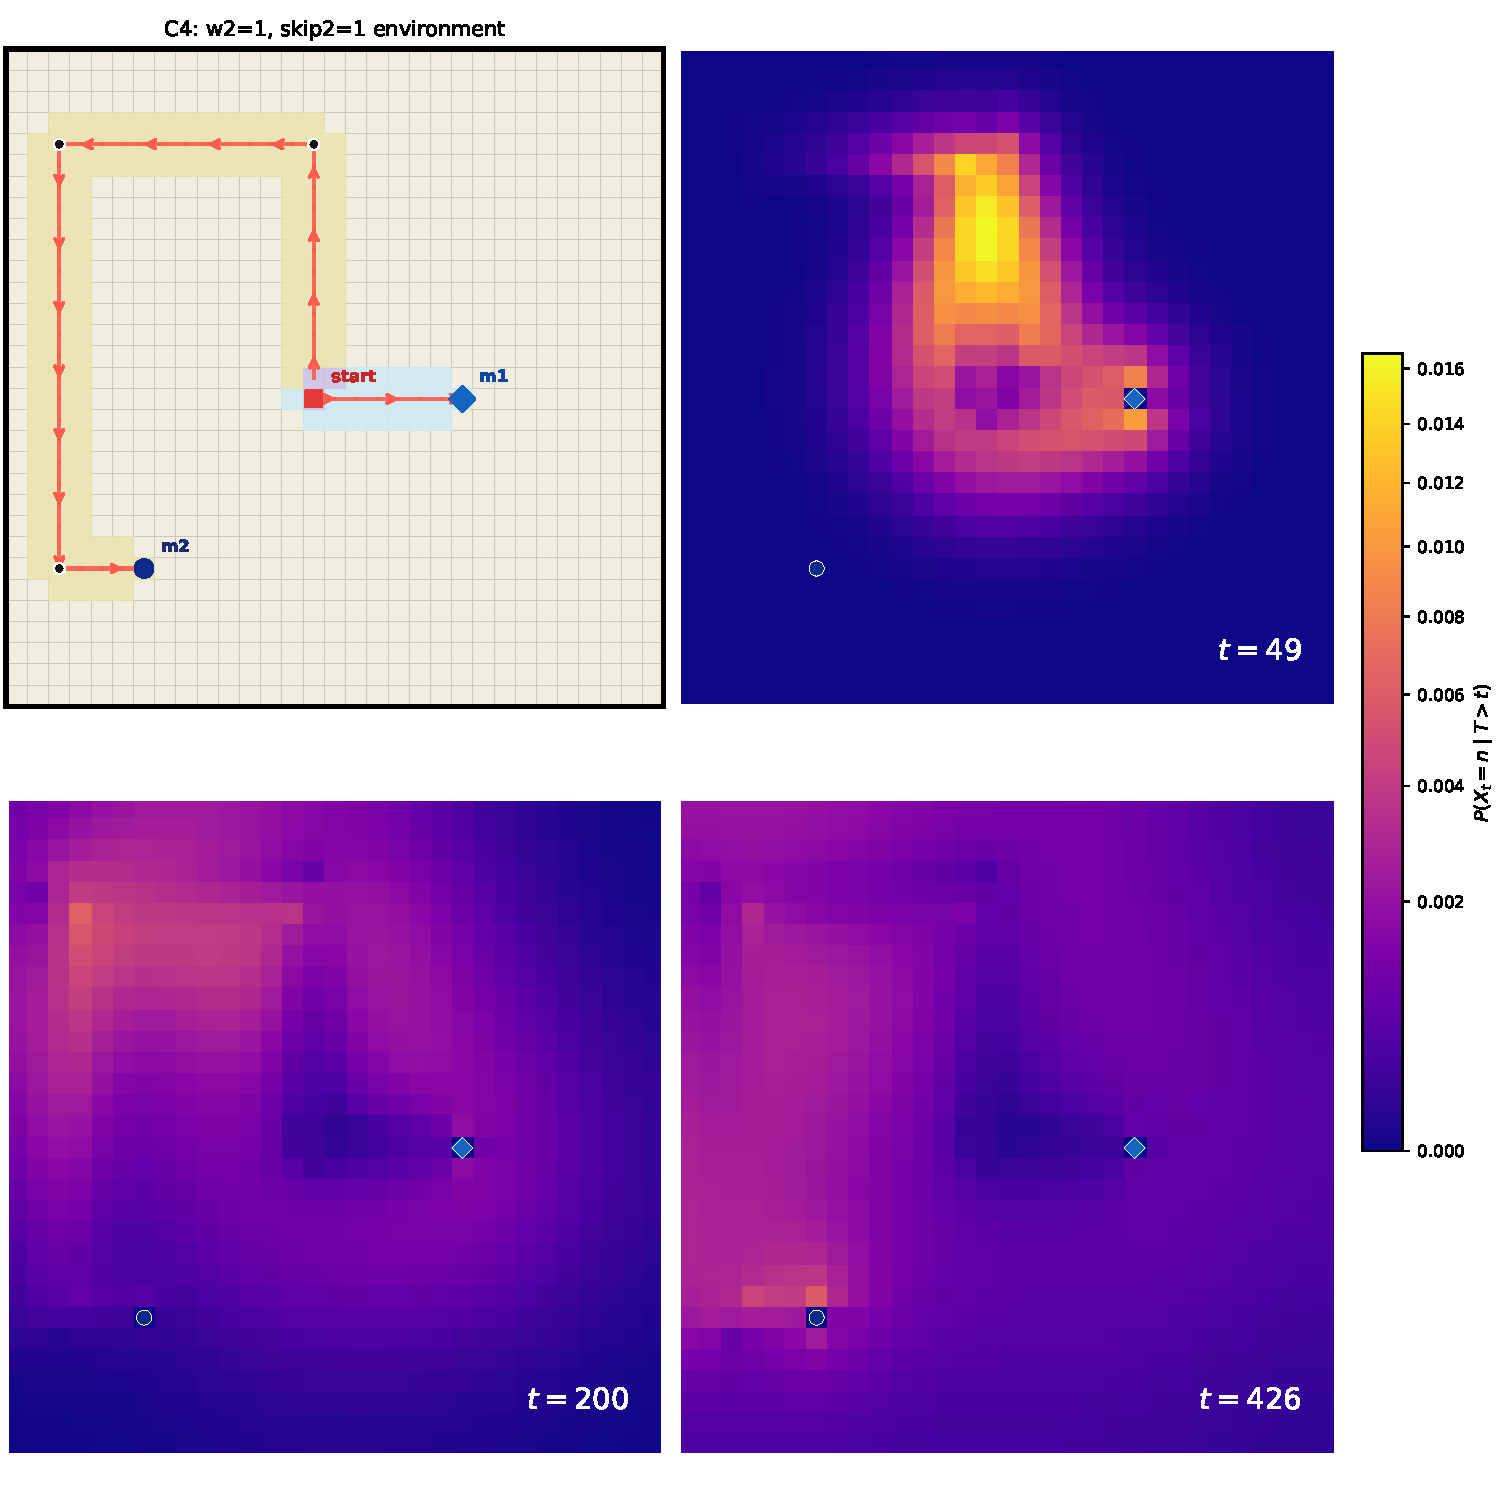
\includegraphics[width=0.82\linewidth]{figures/case_C4_env_heatmap.pdf}
  \caption{C4 environment + three computed conditional occupancy heatmaps ($t=49,200,426$).}
  \label{fig:c4-heat-en}
\end{figure}

\section{Main Results: Total FPT, Splitting, and Hazard}
\begin{figure}[!p]
  \centering
  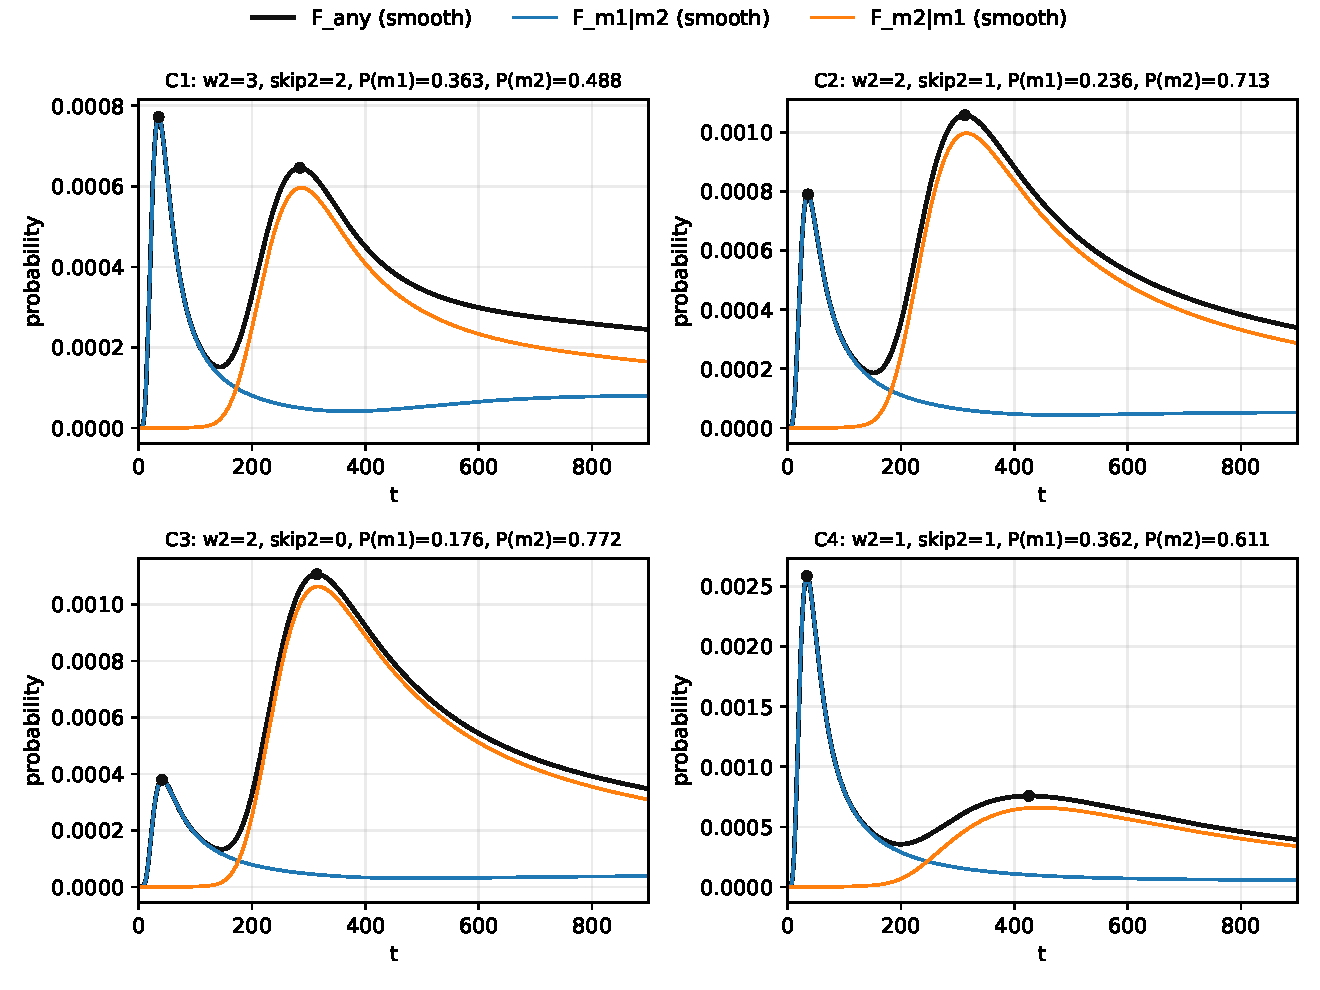
\includegraphics[width=0.98\linewidth]{figures/fpt_grid.pdf}
  \caption{Total first-passage and splitting decomposition for C1--C4. Black: $F_{n_0\to(m_1;m_2)}(t)$; blue/orange: two splitting components.}
  \label{fig:fpt-grid-en}
\end{figure}

\clearpage
\begin{figure}[!p]
  \centering
  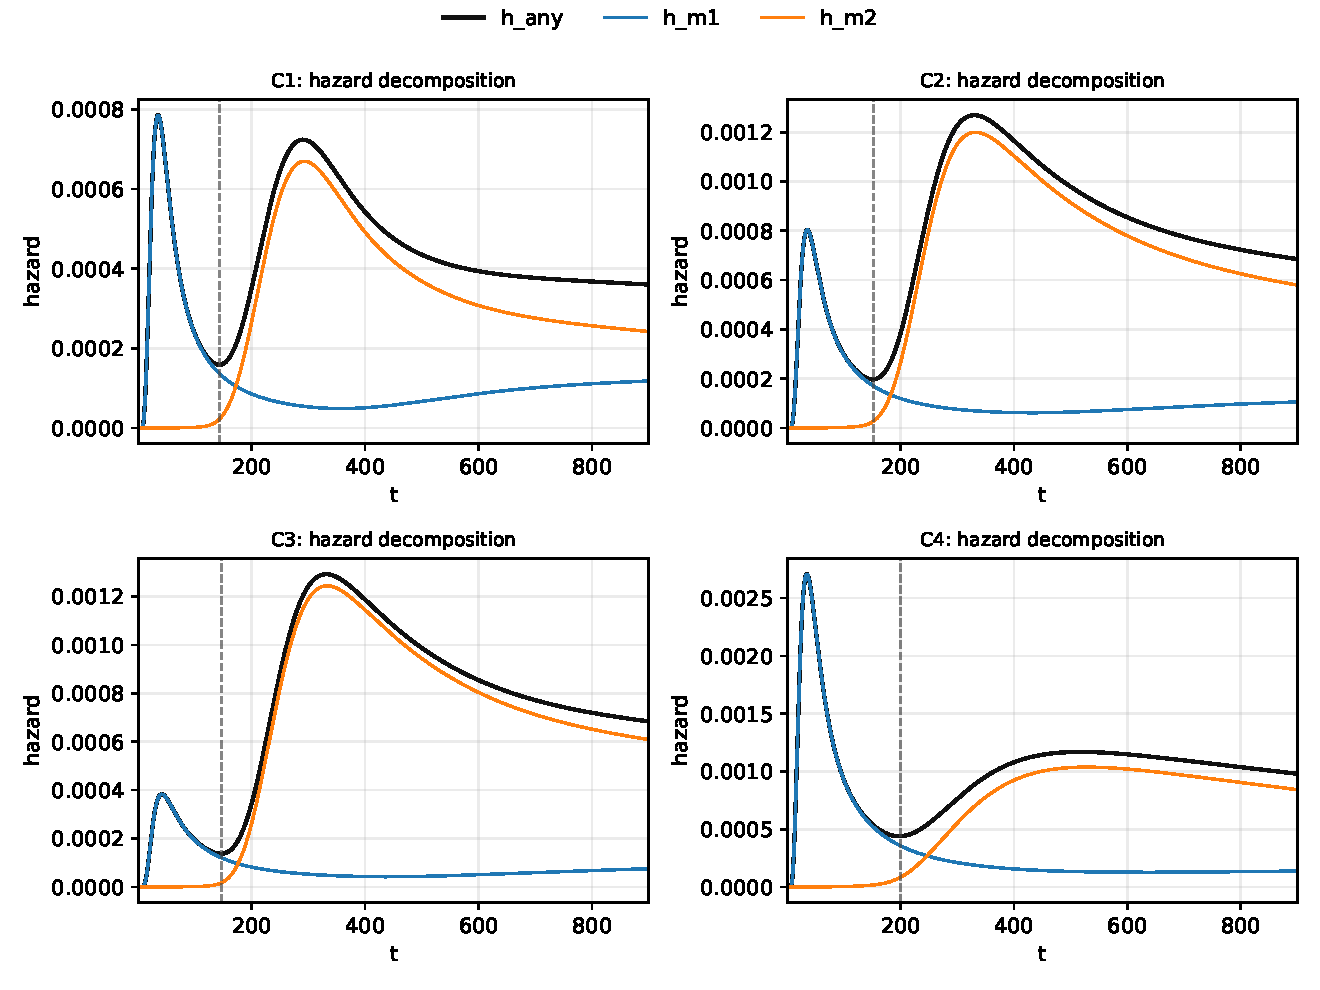
\includegraphics[width=0.98\linewidth]{figures/hazard_grid.pdf}
  \caption{Hazard decomposition $h=h_1+h_2$. Black: total hazard; blue/orange: channel contributions; dashed line: valley time.}
  \label{fig:hazard-grid-en}
\end{figure}
\clearpage

\begin{table}[!htbp]
  \centering
  \footnotesize
  \begin{tabular}{lcccccccc}
\toprule
Case & $w_2$ & skip2 & $t_{p1}$ & $t_{p2}$ & $h_1$ & $h_2$ & $P(m_1)$ & $P(m_2)$ \\
\midrule
C1 & 3 & 2 & 35 & 284 & 7.77e-04 & 6.46e-04 & 0.363 & 0.488 \\
C2 & 2 & 1 & 36 & 313 & 7.94e-04 & 1.06e-03 & 0.236 & 0.713 \\
C3 & 2 & 0 & 41 & 314 & 3.81e-04 & 1.11e-03 & 0.176 & 0.772 \\
C4 & 1 & 1 & 34 & 426 & 2.60e-03 & 7.57e-04 & 0.362 & 0.611 \\
\bottomrule
\end{tabular}
  \caption{Peak locations, peak heights, and splitting weights (with $t_{\max}=6000$ truncation).}
  \label{tab:case-metrics-en}
\end{table}

\begin{table}[!htbp]
  \centering
  \footnotesize
  \begin{tabular}{lcccccc}
\toprule
Case & $t^*_{m_1|m_2}$ & $t^*_{m_2|m_1}$ & $t_v$ & valley/max & absorbed@6000 & tail@6000 \\
\midrule
C1 & 35 & 287 & 143 & 0.194 & 0.851 & 0.149 \\
C2 & 36 & 316 & 152 & 0.176 & 0.949 & 0.051 \\
C3 & 41 & 316 & 146 & 0.120 & 0.948 & 0.052 \\
C4 & 34 & 445 & 200 & 0.137 & 0.973 & 0.027 \\
\bottomrule
\end{tabular}
  \caption{Splitting modal times, valley depth, and absorbed mass at truncation.}
  \label{tab:case-mechanism-en}
\end{table}

\begin{table}[!htbp]
  \centering
  \footnotesize
  \begin{tabular}{lccccc}
\toprule
Case & $t^*_{m_1|m_2}$ & $t^*_{m_2|m_1}$ & $w_{1/2}^{(1)}$ & $w_{1/2}^{(2)}$ & $|\Delta t^*|/(w_{1/2}^{(1)}+w_{1/2}^{(2)})$ \\
\midrule
C1 & 35 & 287 & 25.0 & 141.5 & 1.514 \\
C2 & 36 & 316 & 28.5 & 179.5 & 1.346 \\
C3 & 41 & 316 & 37.5 & 177.0 & 1.282 \\
C4 & 34 & 445 & 26.0 & 319.0 & 1.191 \\
\bottomrule
\end{tabular}
  \caption{Mode-separation score based on mode-distance over summed half-widths.}
  \label{tab:case-separation-en}
\end{table}

\section{Phase Map on $(w_2,\texttt{skip2})$}
\begin{figure}[!htbp]
  \centering
  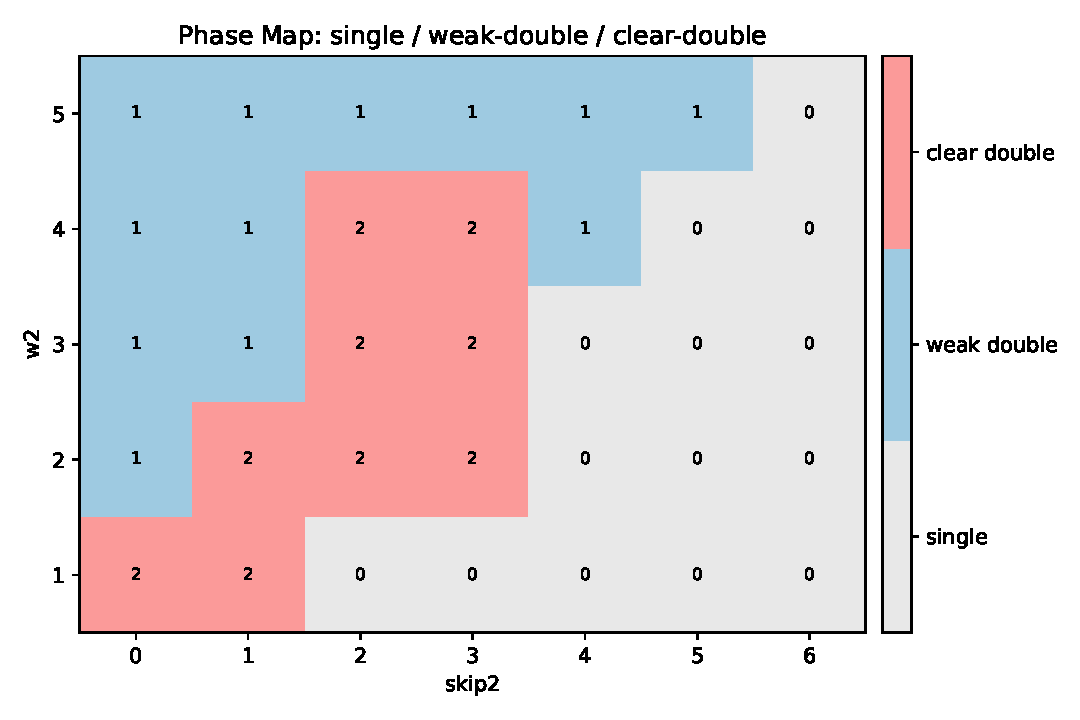
\includegraphics[width=0.68\linewidth]{figures/phase_w2_skip2.pdf}
  \caption{Phase-category map on $(w_2,\texttt{skip2})$: 0=single, 1=weak double, 2=clear double.}
  \label{fig:phase-category-en}
\end{figure}

\begin{figure}[!htbp]
  \centering
  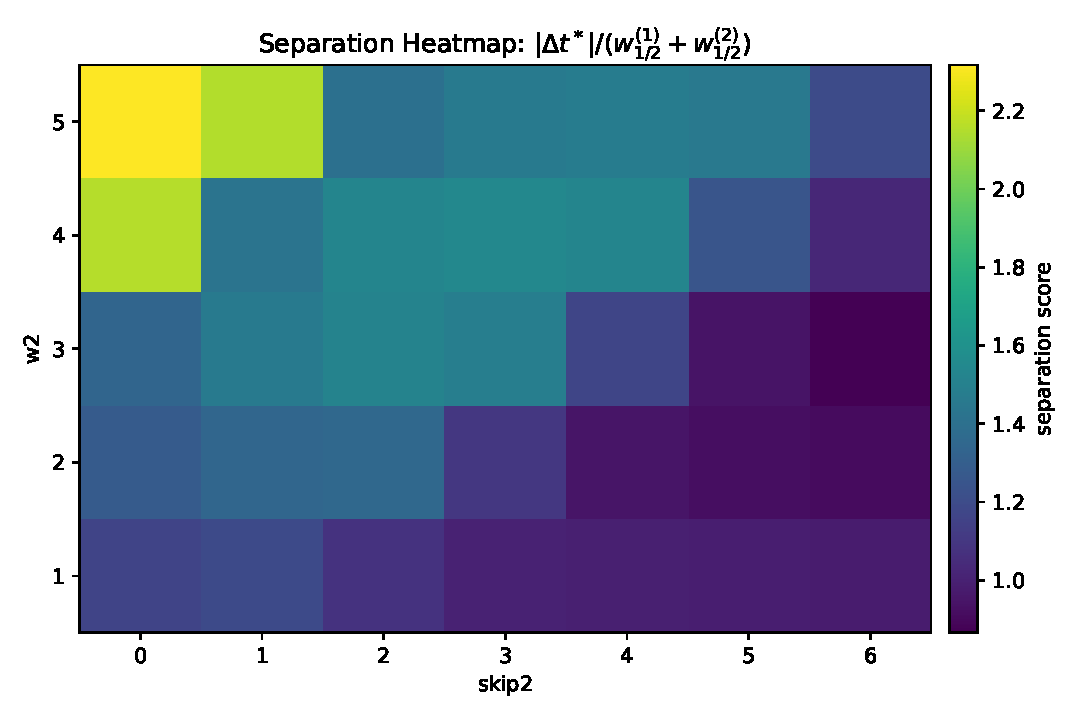
\includegraphics[width=0.68\linewidth]{figures/phase_sep_w2_skip2.pdf}
  \caption{Separation heatmap: $|\Delta t^*|/(w_{1/2}^{(1)}+w_{1/2}^{(2)})$. Brighter means stronger mode separation relative to width.}
  \label{fig:phase-sep-en}
\end{figure}

\section{External Sparse Testset (Double-Peak Cases Only)}
Using
\texttt{external/sparse\_double\_peak\_testset.json},
all 11 sparse-disorder cases were simulated with exact recursion up to $t_{\max}=6000$.
Only phase$>0$ cases are retained in this section.

\begin{table}[!htbp]
  \centering
  \scriptsize
  \begin{tabular}{lp{0.35\linewidth}lcccc}
\toprule
ID & Name & Type & local-bias & sticky & barriers & shortcuts \\
\midrule
S02 & corridor thin w2 1 skip2 0 & corridor\_model & 160 & 0 & 0 & 0 \\
S03 & centerline only bias fast and slow & explicit\_bias\_list & 54 & 0 & 0 & 0 \\
\bottomrule
\end{tabular}
  \caption{Configuration statistics for retained sparse-testset double-peak cases.}
  \label{tab:sparse-configs-en}
\end{table}

\begin{table}[!htbp]
  \centering
  \scriptsize
  \begin{tabular}{lccccccc}
\toprule
ID & $t_{p1}$ & $t_{p2}$ & valley/max & $P(m_1)$ & $P(m_2)$ & sep-score & phase \\
\midrule
S02 & 38 & 436 & 0.235 & 0.233 & 0.740 & 1.17 & 2 \\
S03 & 38 & 925 & 0.217 & 0.411 & 0.511 & 0.92 & 1 \\
\bottomrule
\end{tabular}
  \caption{Double-peak metrics for retained sparse-testset cases.}
  \label{tab:sparse-metrics-en}
\end{table}

\begin{figure}[!p]
  \centering
  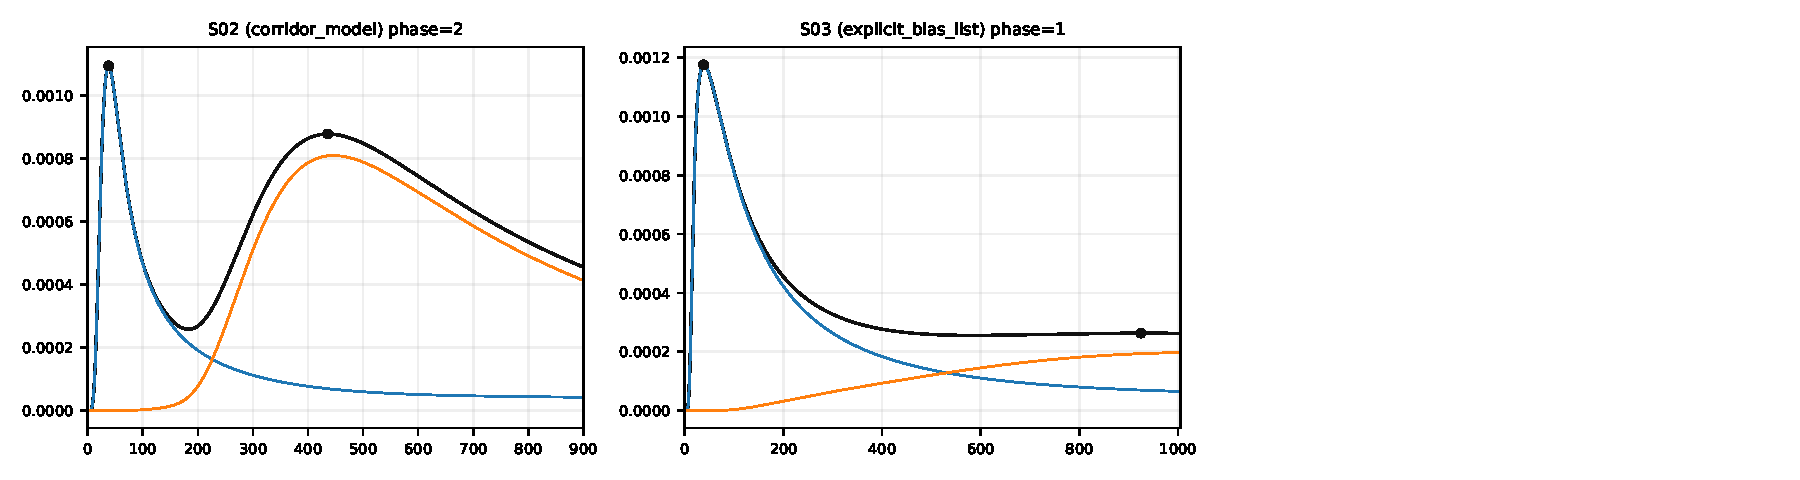
\includegraphics[width=0.98\linewidth]{figures/sparse_testset_fpt_grid.pdf}
  \caption{Retained sparse-testset overview (currently S02 clear-double and S03 weak-double).}
  \label{fig:sparse-fpt-grid-en}
\end{figure}

\begin{figure}[!p]
  \centering
  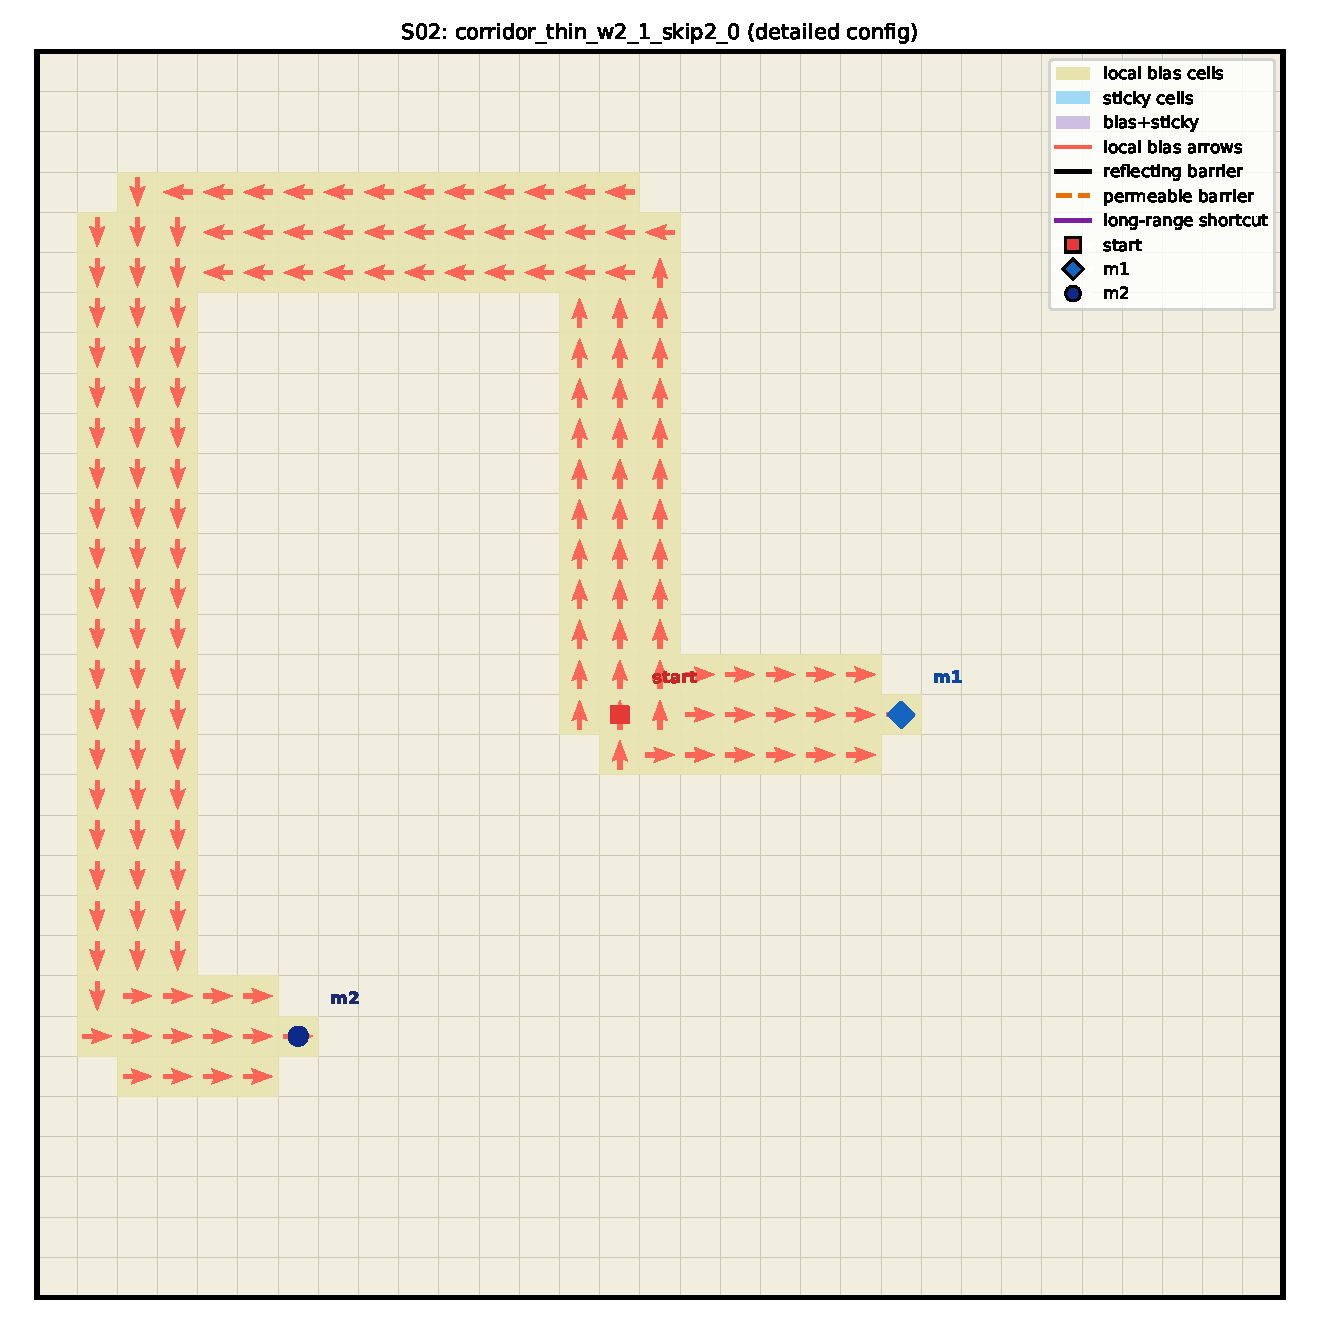
\includegraphics[width=0.95\linewidth]{figures/sparse_S02_config_detailed.pdf}
  \caption{S02 detailed configuration: all biased cells and all arrows shown explicitly.}
  \label{fig:sparse-s02-config-en}
\end{figure}

\begin{figure}[!p]
  \centering
  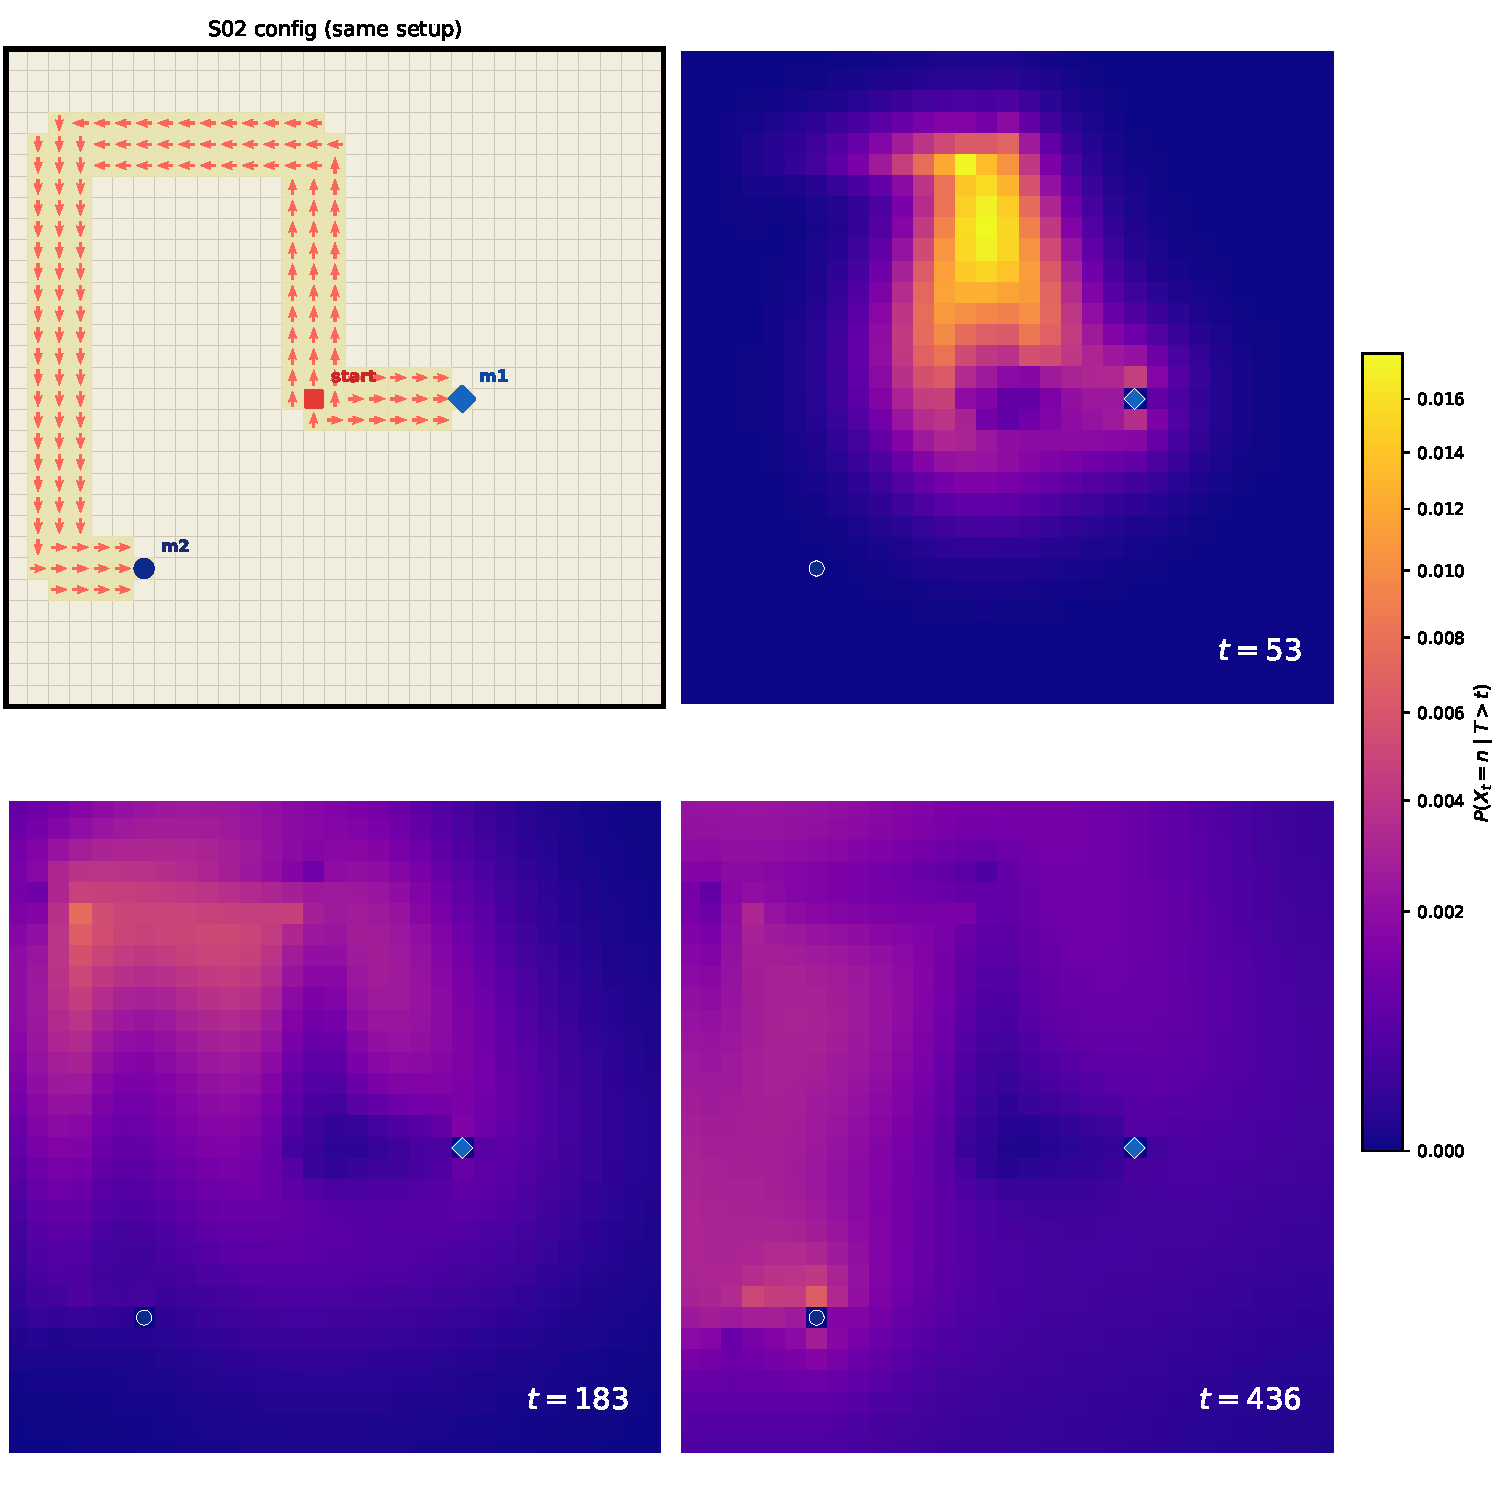
\includegraphics[width=0.95\linewidth]{figures/sparse_S02_env_heatmap.pdf}
  \caption{S02 configuration + three-stage conditional occupancy heatmaps (early peak, valley window, late peak window).}
  \label{fig:sparse-s02-heat-en}
\end{figure}

\begin{figure}[!p]
  \centering
  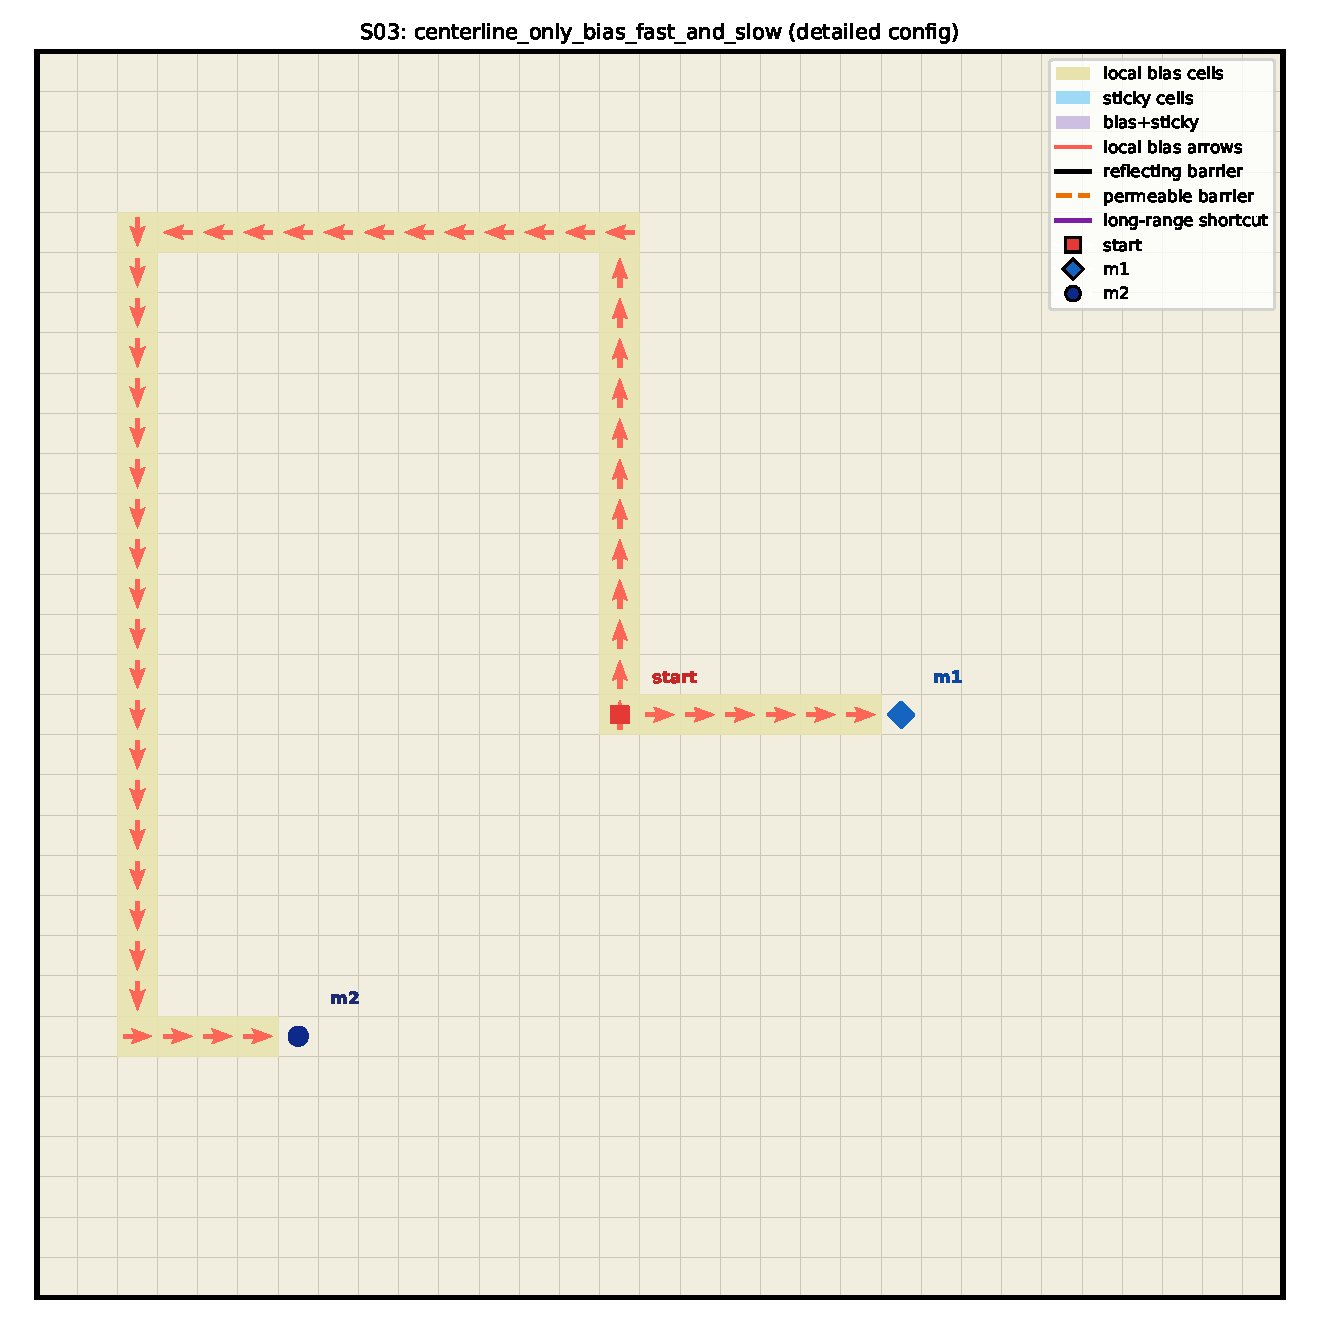
\includegraphics[width=0.95\linewidth]{figures/sparse_S03_config_detailed.pdf}
  \caption{S03 detailed configuration: centerline-only sparse bias layout.}
  \label{fig:sparse-s03-config-en}
\end{figure}

\begin{figure}[!p]
  \centering
  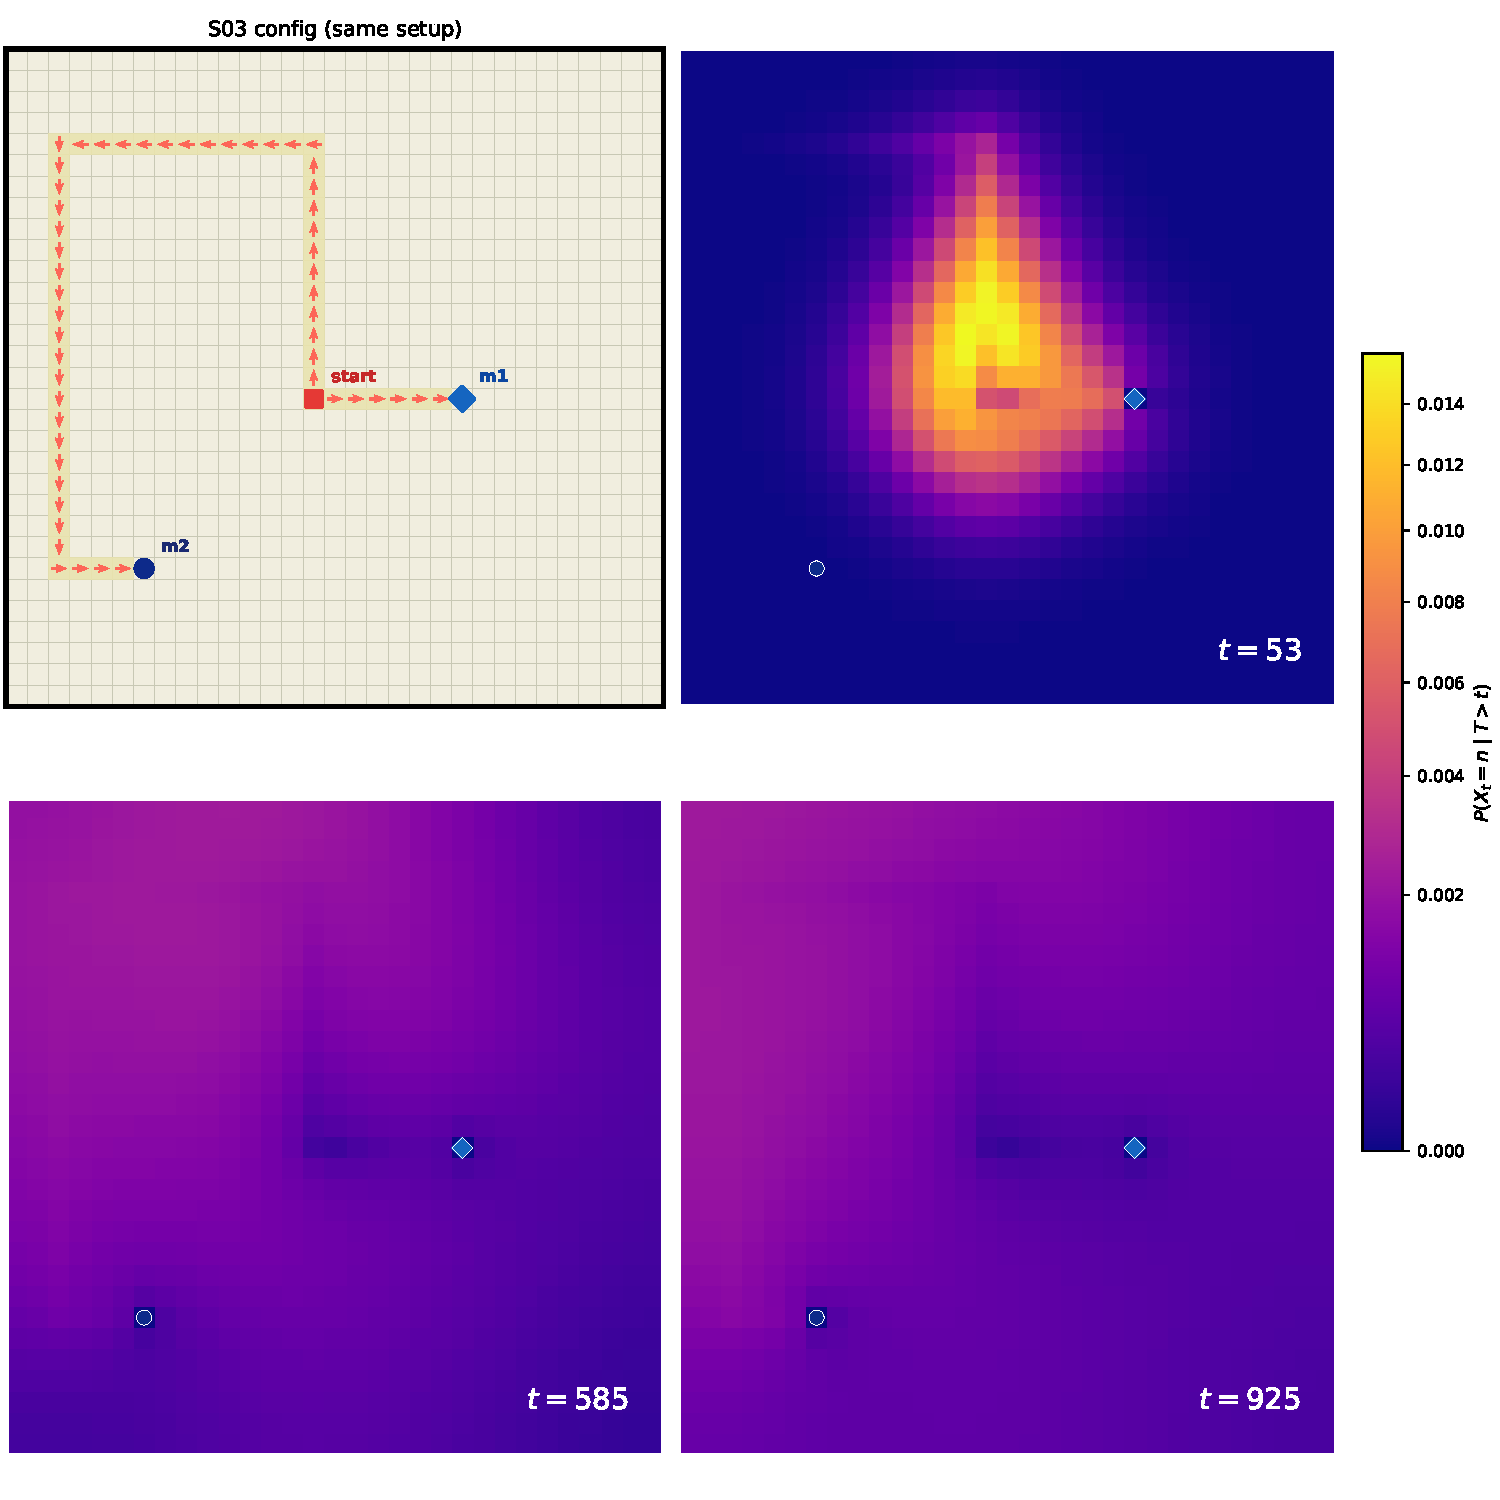
\includegraphics[width=0.95\linewidth]{figures/sparse_S03_env_heatmap.pdf}
  \caption{S03 configuration + three-stage conditional occupancy heatmaps (weak-double behavior).}
  \label{fig:sparse-s03-heat-en}
\end{figure}

\section{Reproducibility}
\begin{verbatim}
cd reports/grid2d_two_target_double_peak
.venv/bin/python code/two_target_2d_report.py
latexmk -pdf -interaction=nonstopmode -halt-on-error -auxdir=build \
  -emulate-aux-dir grid2d_two_target_double_peak_en.tex
\end{verbatim}

Core outputs used by this report:
\begin{itemize}
  \item \texttt{data/case\_summary.json}
  \item \texttt{data/sparse\_testset\_results.json}
  \item \texttt{data/scan\_w2\_skip2.csv}, \texttt{data/scan\_w2\_skip2.json}
  \item \texttt{outputs/C1\_fpt.csv} -- \texttt{outputs/C4\_fpt.csv}
  \item \texttt{outputs/S02\_external\_fpt.csv}, \texttt{outputs/S03\_external\_fpt.csv}
\end{itemize}

\clearpage
\section*{Appendix: Full Arrow-Field Maps (One Arrow per Biased Cell)}
\begin{figure}[!p]
  \centering
  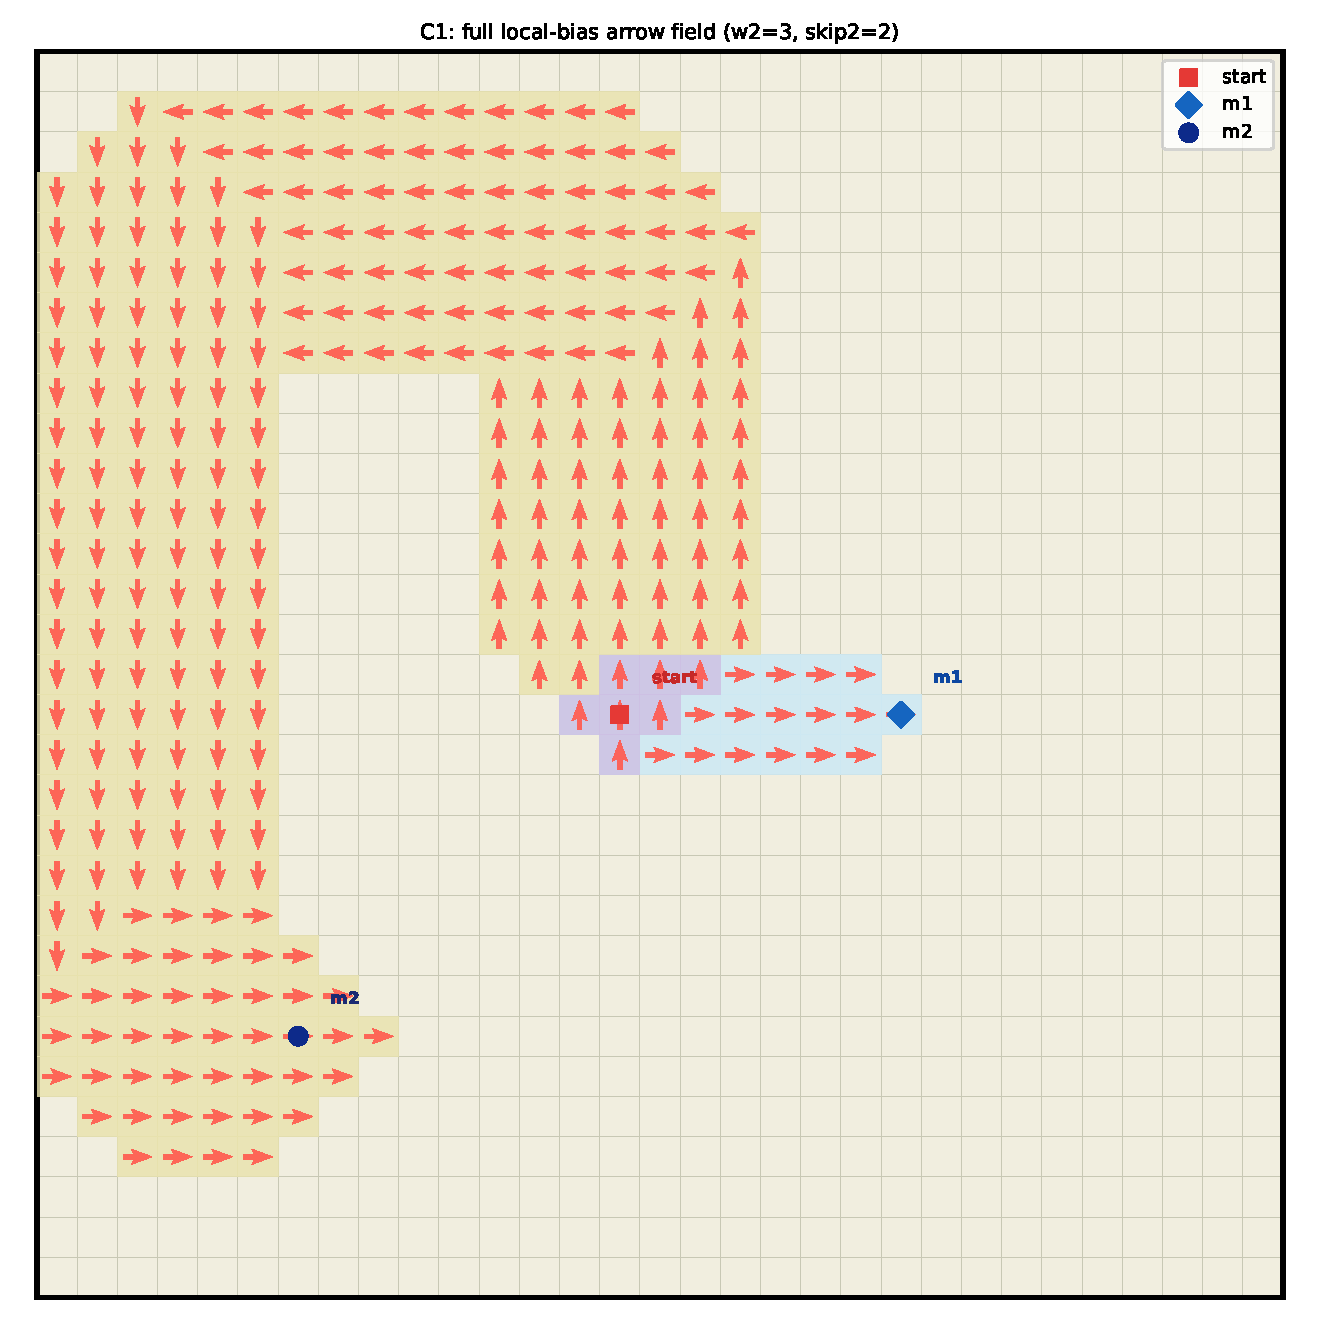
\includegraphics[width=0.95\linewidth]{figures/case_C1_arrowfield.pdf}
  \caption{C1 full local-bias arrow field ($w_2=3,\ \texttt{skip2}=2$).}
  \label{fig:c1-arrowfield-en}
\end{figure}

\begin{figure}[!p]
  \centering
  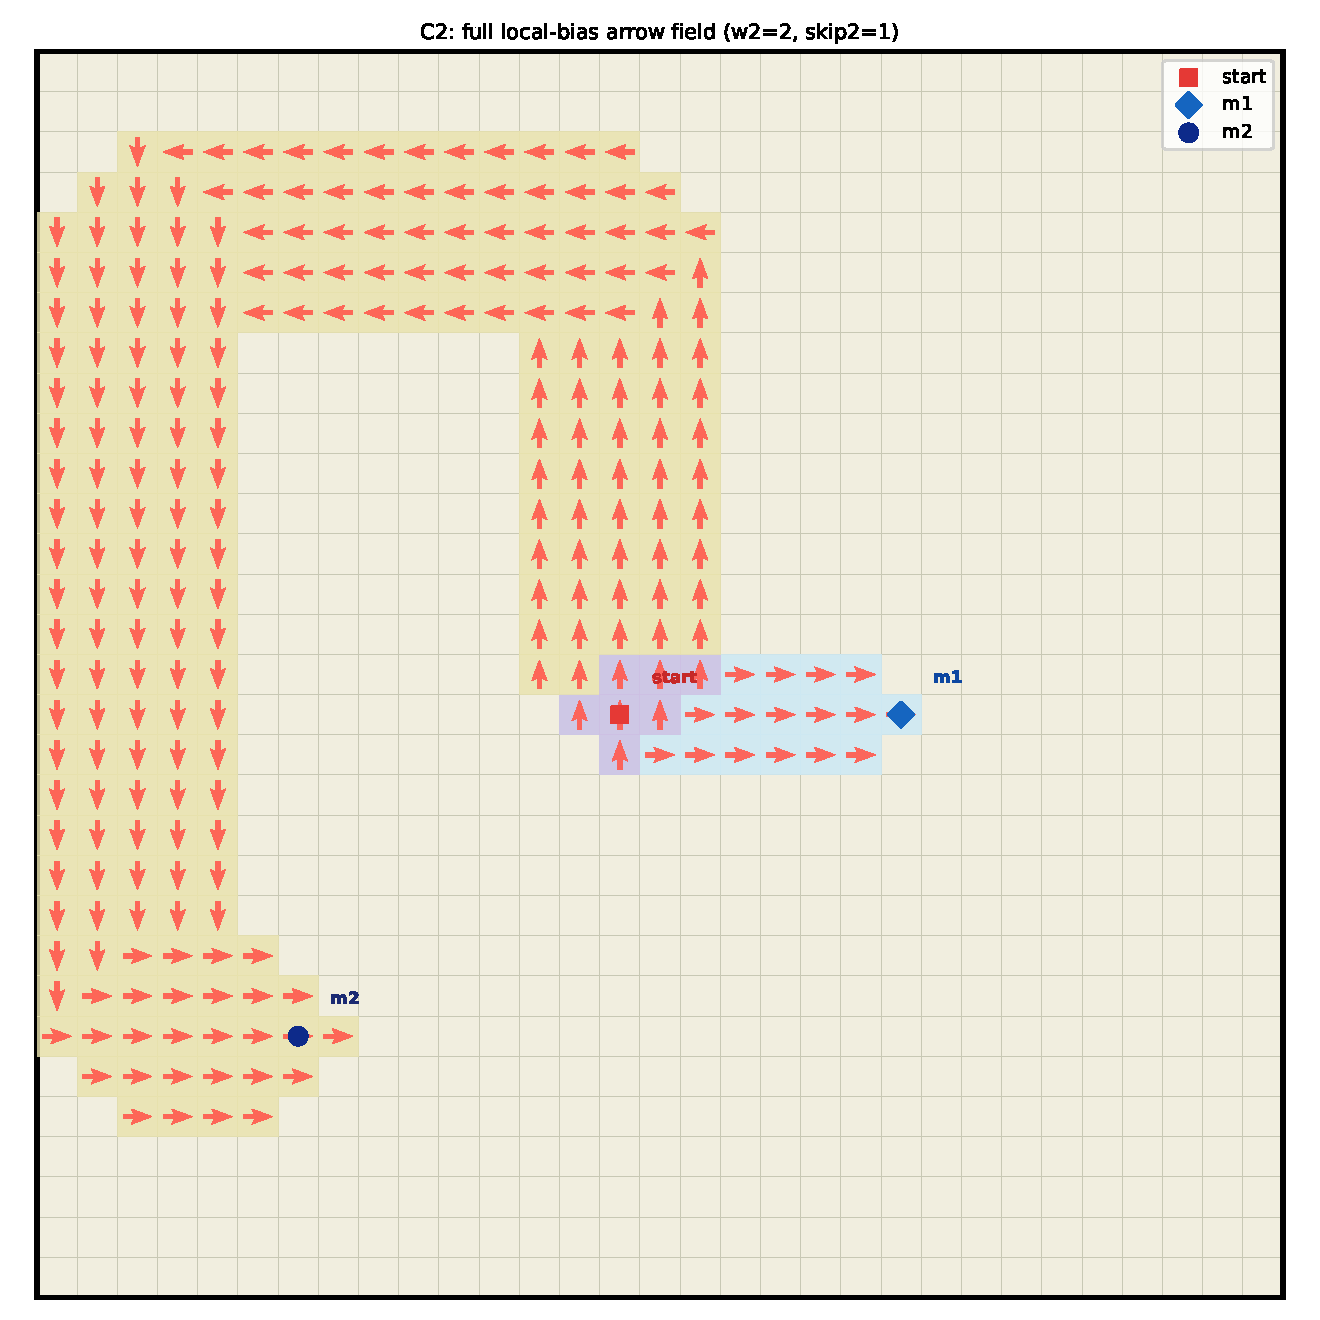
\includegraphics[width=0.95\linewidth]{figures/case_C2_arrowfield.pdf}
  \caption{C2 full local-bias arrow field ($w_2=2,\ \texttt{skip2}=1$).}
  \label{fig:c2-arrowfield-en}
\end{figure}

\begin{figure}[!p]
  \centering
  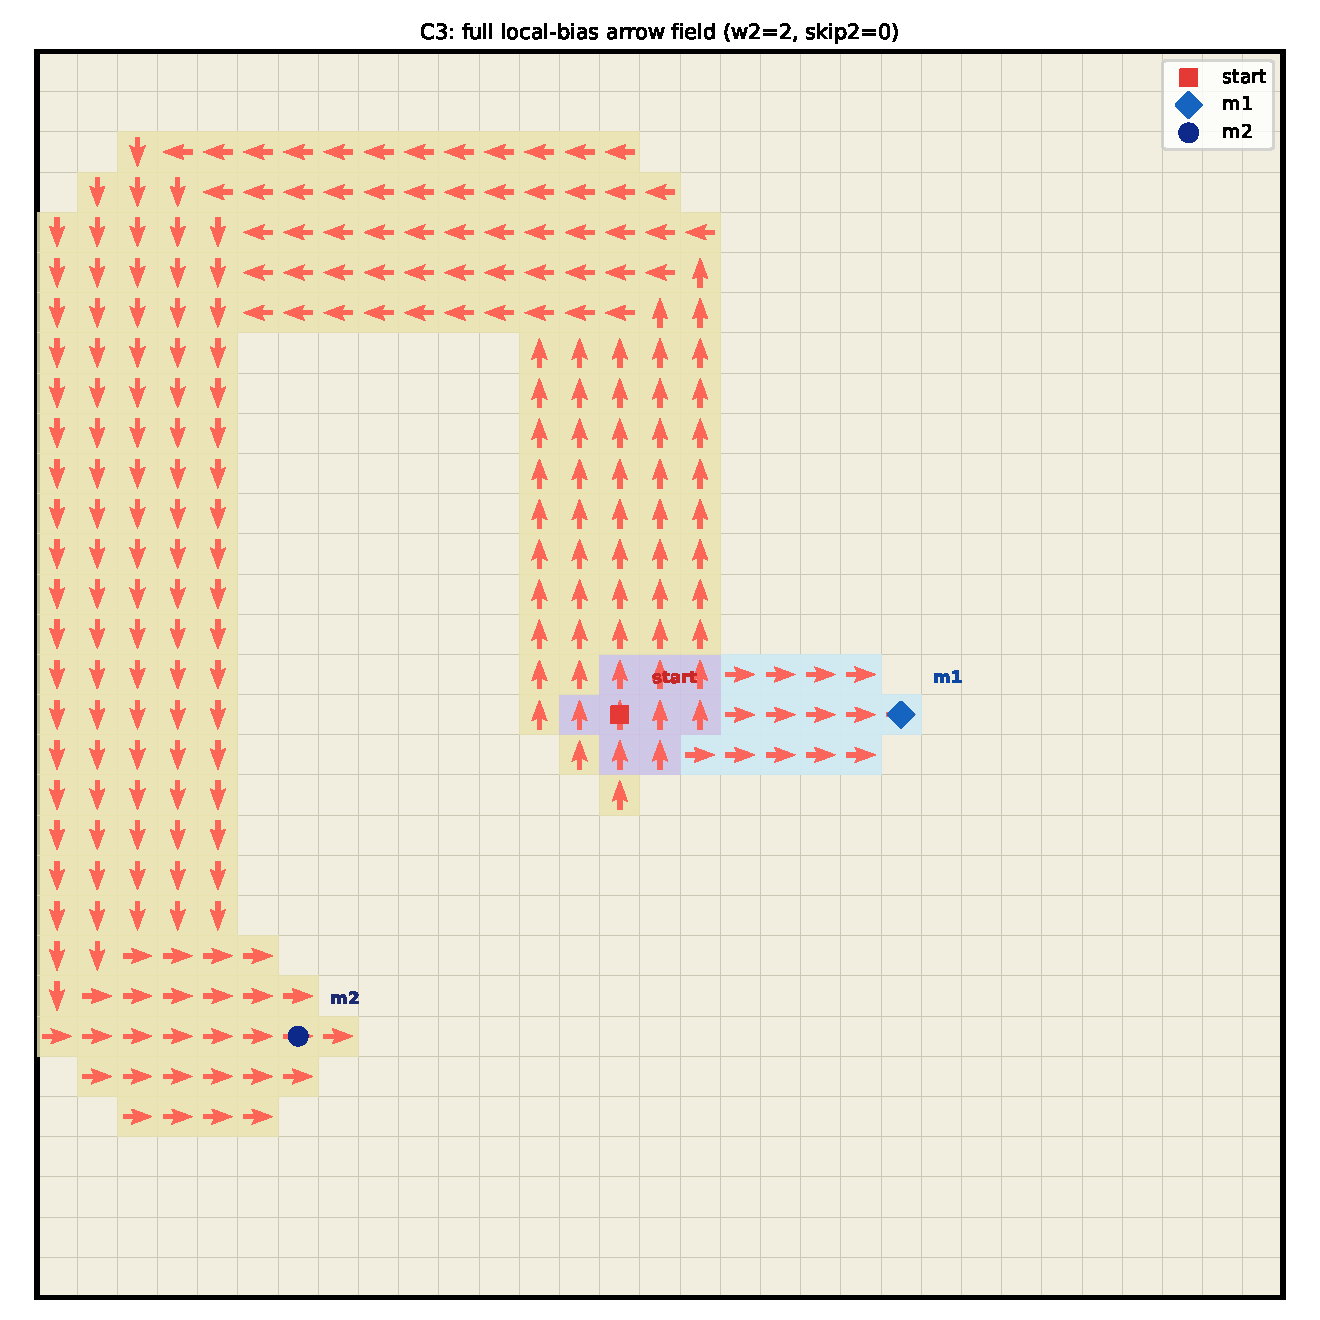
\includegraphics[width=0.95\linewidth]{figures/case_C3_arrowfield.pdf}
  \caption{C3 full local-bias arrow field ($w_2=2,\ \texttt{skip2}=0$).}
  \label{fig:c3-arrowfield-en}
\end{figure}

\begin{figure}[!p]
  \centering
  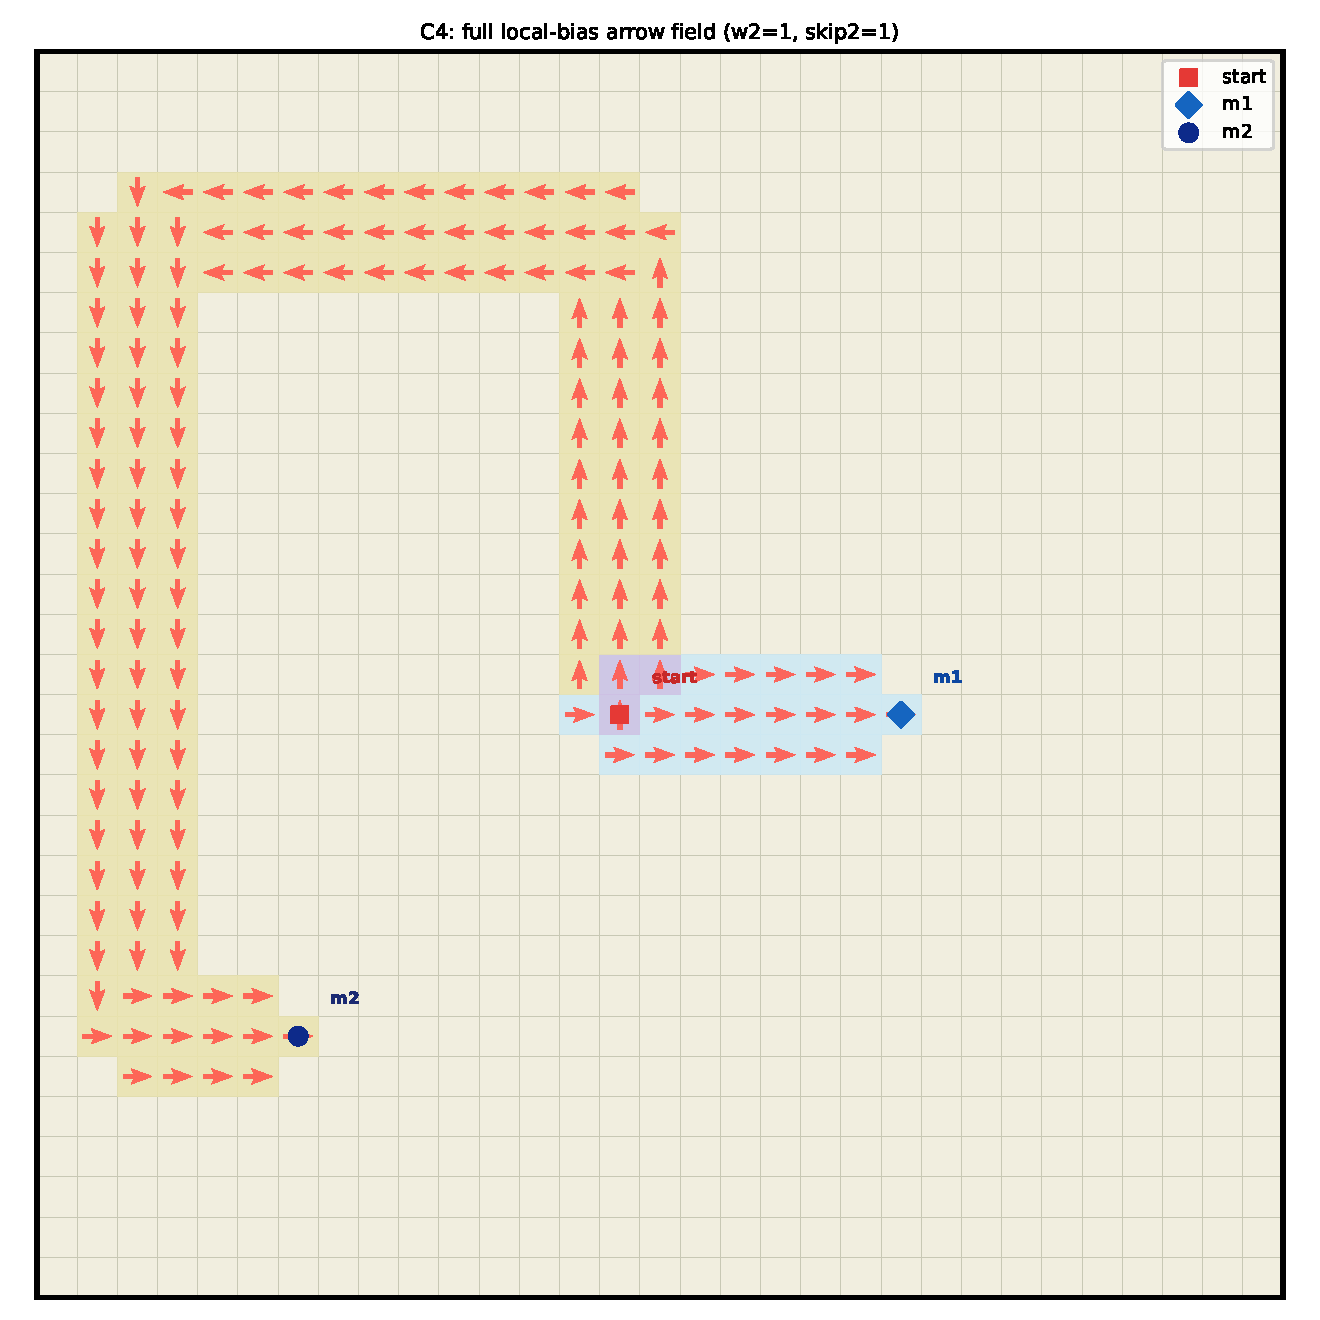
\includegraphics[width=0.95\linewidth]{figures/case_C4_arrowfield.pdf}
  \caption{C4 full local-bias arrow field ($w_2=1,\ \texttt{skip2}=1$).}
  \label{fig:c4-arrowfield-en}
\end{figure}

\end{document}
